\chapter{Central potential}

In the following, we investigate stationary states in the central potential $V (\vec{r}) = V (r)$, that is, in problems with rotationally symmetric potentials.
The Hamiltonian is
%公式 5.1
\begin{equation}
    H=\frac{p^{2}}{2 m}+V(r)
    \end{equation}
and we examine the eigenvalue problem
%公式 5.2
\begin{equation}
    H \Psi(\vec{r})=E \Psi(\vec{r})
    \end{equation}
It is $V = V (r)$ but $\Psi=\Psi(\vec{r})$, which means that the wave function $\Psi$ also has structure in the angle coordinates. The rotational symmetry $[H,U_{\vec{w}}]=0,U_{\vec{w}}\in\mathcal{SO}(3)$, allows us to diagonalize $H, L^2$ and $L_z$ at the same time, simplifying the solution of the problem. \\\\
The situation is similar to that in mechanics: each symmetry corresponds to a size obtained, in the present problem this is the invariance under translations in time and under rotations; the associated conserved quantities are the energy E and the angular momentum $\vec{L}$. These conservation laws are very helpful in solving the mechanical problem. \\\\
The same symmetries in quantum mechanics give us a sharp (received) energy and an obtained angular momentum because $[H, \vec{L}] = 0$. However, a difference occurs due to the non-commutability of the three angular momentum components; although we can set $\vec{L}$ in any direction (we call it the z-direction), it follows that $[L_i, L_j] = i\hbar \varepsilon_{ijk}L_k\neq 0$ that we can not set all three components simultaneously. Thus, the four obtained sizes in mechanics correspond to only three quantum numbers $E$ (to the Hamiltonian $H, l$ (to the angular momentum $L^2$), and $m$ (to the angular momentum component $L_z$) in quantum mechanics.)\\\\
Technically, the solution of the problem is simplified by just Solving the angular problem by reducing the rotation group in the Hilbert space, we can solve the remaining radial problem in each sector in a fixed way.
We go to spherical coordinates so that we can directly exploit the rotational symmetry.

\section{Eigenvalue problem in spherical coordinates}
It is
%公式 5.3
\begin{equation}
\begin{aligned} L^{2} &=\varepsilon_{i j k} x_{j} p_{k} \varepsilon_{i l m} x_{l} p_{m} \\ &=\left(\delta_{j l} \delta_{k m}-\delta_{j m} \delta_{k l}\right) x_{j} p_{k} x_{l} p_{m} \\ &\left.=x_{j l} \delta_{k m}-\delta_{j m} \delta_{k l}\right) x_{j} p_{k} x_{l} p_{m} \\ &=x_{j} p_{k} x_{j} p_{k}-x_{j} p_{k} x_{k} p_{j} \\ &=x_{j}\left(x_{j} p_{k}-i \hbar \delta_{j k}\right) p_{k}-x_{j}\left(x_{k} p_{k}-3 i \hbar\right) p_{j} \\ &=x_{j} x_{j} p_{k} p_{k}-i \hbar x_{j} p_{j}-x_{j} x_{k} p_{k} p_{j}+3 i \hbar x_{j} p_{j} \\ &=r^{2} p^{2}-i \hbar \vec{r} \cdot \vec{p}-\underbrace{x_{j}\left(p_{j} x_{k}+i \hbar \delta_{j k}\right) p_{k}}_{(\vec{r} \cdot \vec{p})^{2}+t \hbar \vec{r} \cdot \vec{p}} \\ &=r^{2} p^{2}-(\vec{r} \cdot \vec{p})^{2}+i \hbar \vec{r} \cdot \vec{p} \end{aligned}
\end{equation}
Classically, $L^2=r^2p^2-(\vec{r}\cdot\vec{p})^2$ for the proof, calculate directly or use the $\operatorname{lim}\hbar\rightarrow 0$ of (5.3). It is
%公式
$$
\vec{\nabla}=\left(\partial_{x}, \partial_{y}, \partial_{z}\right) \rightarrow\left(\partial_{r}, \frac{1}{r \sin \theta} \partial_{\varphi}, \frac{1}{r} \partial_{\theta}\right)
$$
and
%公式 5.4
\begin{equation}
    \vec{r} \cdot \vec{p}=-i \hbar \vec{r} \cdot \vec{\nabla}^{\vec{r}=r \hat{e}_{r}}-i \hbar r \partial_{r}
    \end{equation}
the projection from $\vec{p}$ to $\vec{r}$. With (5.3) we get the kinetic energy (or the Laplace operator $\Delta$) in spherical coordinates,
%公式 5.5
\begin{equation}
\begin{aligned} p^{2} &=-\hbar^{2} \nabla^{2}=-\hbar^{2} \Delta=\frac{1}{r^{2}}\left(\vec{L}^{2}+(\vec{r} \cdot \vec{p})^{2}-i \hbar \vec{r} \cdot \vec{p}\right) \\ &=-\frac{\hbar^{2}}{r^{2}}\left[\left(r \partial_{r}\right)^{2}+r \partial_{r}\right]+\frac{L^{2}}{r^{2}} \\ &=p_{r}^{2}+\quad \frac{L^{2}}{r^{2}} \end{aligned}
\end{equation}
$p_r$ is asymptotically the radial component of the momentum and has the forms
% 5.6
\begin{equation}
    p_{r}=-i \hbar r^{-1}\left(\partial_{r} r\right)=-i \hbar\left(\partial_{r}+\frac{1}{r}\right)
    \end{equation}
The operator $p^2_r$ can then be written as follows,
%公式 5.7
\begin{equation}
\begin{aligned} p_{r}^{2} &=-\hbar^{2}\left(\partial_{r}^{2}+\frac{2}{r} \partial_{r}\right)=-\hbar^{2}\left(\partial_{r}^{2}+\frac{\operatorname{dim}-1}{r} \partial_{r}\right) \\ &=-\hbar^{2}\left(\frac{1}{r} \partial_{r} r \partial_{r}+\frac{1}{r} \partial_{r}\right) \\ &=-\hbar^{2}\left(\frac{1}{r} \partial_{r} r\right)^{2}=-\hbar^{2}\left(\frac{1}{r} \partial_{r}^{2} r\right)=-\hbar^{2}\left(\frac{1}{r^{2}} \partial_{r} r^{2} \partial_{r}\right) \end{aligned}
\end{equation}
It is $[r, p_r] = i \hbar$, that is, $p_r$ is canonically conjugate to $r$. The eigenvalue problem takes the following form in spherical coordinates,
%公式 5.8
\begin{equation}
    \left[-\frac{\hbar^{2}}{2 m}\left(\partial_{r}^{2}+\frac{2}{r} \partial_{r}\right)+\frac{L^{2}}{2 m r^{2}}+V(r)\right] \Psi(\vec{r})=E \Psi(\vec{r})
    \end{equation}
The angular coordinates are in $L^2$, see (4.40) and for the Laplace operator $\Delta$ is given
%公式 5.9
\begin{equation}
    \Delta=\partial_{r}^{2}+\frac{2}{r} \partial_{r}+\underbrace{\frac{1}{r^{2} \sin ^{2} \theta} \partial_{\varphi}^{2}+\frac{1}{r^{2} \sin \theta} \partial_{\theta}\left(\sin \theta \partial_{\theta}\right)}_{-L^{2} / \hbar^{2} r^{2}}
    \end{equation}
But since we have already solved the angle problem $L^2 Y_{l, m}=\hbar^2 l(l+1)Y_{l,m}$, it makes no sense to go to (5.9). The rotational symmetry $V = V (r)$ separates the angular and radial coordinates
%公式
$$
\begin{aligned} \Psi(r, \theta, \varphi) &=R(r) Y_{l, m}(\theta, \varphi) \\ L^{2} Y_{l, m} &=\hbar^{2} l(l+1) Y_{l, m} \end{aligned}
$$
and we can immediately go over to the radial problem,
% 5.10
\begin{equation}
    \left[-\frac{\hbar^{2}}{2 m}\left(\partial_{r}^{2}+\frac{2}{r} \partial_{r}\right)+\frac{\hbar^{2} l(l+1)}{2 m r^{2}}+V(r)\right] R(r)=E R(r)
    \end{equation}
To obtain the form of a 1-D Schrodinger equation we write the radial function $R (r)$ in the form
%公式 5.11
\begin{equation}
    R(r)=\frac{u(r)}{r}
    \end{equation}
and get the equation
%%公式 5.12
\begin{equation}
    \left[-\frac{\hbar^{2}}{2 m} \partial_{r}^{2}+\underbrace{\frac{\hbar^{2} l(l+1)}{2 m r^{2}}+V(r)}_{V_{\mathrm{eff}}(r)}\right] u(r)=E u(r)
    \end{equation}
Only for $l = 0$, angular momentum zero, is $V_{\text{eff}} (r) = V (r)$. Otherwise, in addition to $V (r)$, the repulsive potential $V_l (r) = \hbar^2l(l+1) / 2m r^2$ acts on the particle, the well-known centrifugal barrier, see figure 5.1. We will see that, because of this term, $\Psi(r)\propto r^l$ is suppressed for $r \rightarrow 0$ and the particle is displaced from $r = 0$. The equation (5.12)
%图 5.1
\begin{figure}[ht]
    \begin{minipage}{0.5\textwidth}
        \centering
        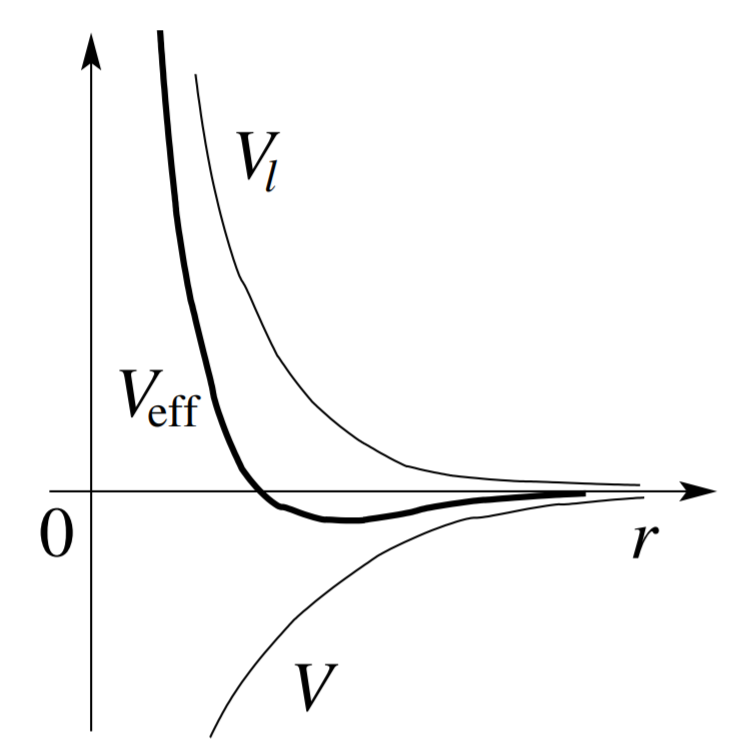
\includegraphics[scale=1]{5_1.PNG}
    \end{minipage}
    \begin{minipage}{0.5\textwidth}
        \captionsetup{font={Large}}
        \caption{The angular momentum generates
        the potential barrier $V_l=\hbar^2l(l+1)/2mr^2$ and displaces the wave function from the environment of origin. The potential $V (r)$ combines with $V_l (r)$ to be effective potential $V_{\text{eff}} (r)$.}
    \end{minipage}
\end{figure}
corresponds to a 1-D Schr¨odinger problem with $V (x <0) = \infty, V (x> 0) = V (x = r)$; for an attractive potential, the typical situation in Figure 5.2 is sketched. Conversely, the symmetric extension $V (x <0) = V (| x | = r)$ gives us a typical 1-D problem. In 1-D, every attractive potential (with $V (| x |\rightarrow \infty) \rightarrow 0, V (0) <0)$ binds at least one (in $x$ direction, $V (x) = V (| x |)$ is invariant under $x \rightarrow -x$) state. Now consider the dim = 3, $l = 0$ problem. Then $u (0) = 0$, and thus $u$ odd. It follows that the attractive potential in dim = 3 must have a minimum strength so that it can bind a state, cf. the discussion in section 3.3 (particles in the pot).\\\\
A dimensional estimate gives the condition $V_0>\hbar^2/2mr_0^2$ for a bound state in the $l = 0$ sector. In addition, the centrifugal barrier counteracts the formation of bound states for ¨$l> 0$. Next we investigate the behavior of $u (r)$ and thus of the wave function $ \Psi (\vec{r}$) in the limits $r \rightarrow 0$ and $r \rightarrow \infty$.
% 5.2
\begin{figure}[ht]
    \begin{minipage}{0.6\textwidth}
        \centering
        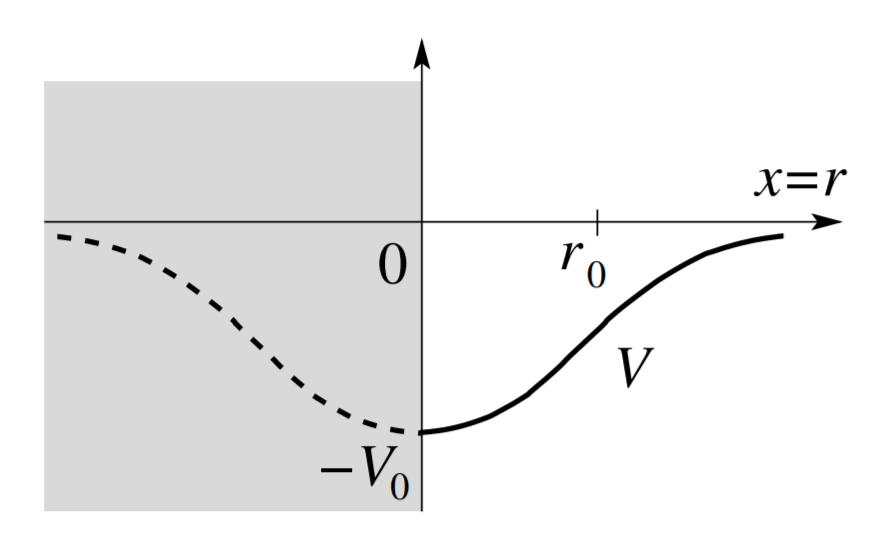
\includegraphics[scale=1]{5_2.PNG}
    \end{minipage}
    \begin{minipage}{0.3\textwidth}
        \captionsetup{font={Large}}
        \caption{The centrally symmetric potential problem leaves to a equivalent half-sided 1D problem (with $r=x\geq 0$), here for illustrates an attractive potential.}
    \end{minipage}
\end{figure}
Limit case $r \rightarrow 0$ For ¨$V (r) \propto 1 / r^{2-\varepsilon}, \varepsilon> 0$, the leading terms (¨$l> 0$) of the differential equation (5.12) are given
%公式 5.13
\begin{equation}
    \left[-\frac{\hbar^{2}}{2 m} \partial_{r}^{2}+\frac{\hbar^{2} l(l+1)}{2 m r^{2}}\right] u(r)=0
    \end{equation}
This results in the following solutions for u (r),
%公式 5.14
\begin{equation}
u(r) \propto\left\{\begin{array}{ll}{r^{l+1}} & {\leftarrow \text { reguläre Lösung }} \\ {r^{-l}} & {\leftarrow \text { nicht normierbar }}\end{array}\right.
\end{equation}
For ¨$l = 0, u$ has to disappear at $r = 0$ (proof to absurdity): Let $u (0) = u_0 \neq 0$, then $\Psi (\vec{r}) \propto u_0 / r$ at $0$ and $\nabla^2$ generates a δ-function at 0 (the function $1 / r$ is just the Green function for the Laplace problem, $\nabla^2 (1 / r) = -4π\delta (\vec{r})$, to be checked using the theorem of Gauss). This $\delta$-function remains uncompensated in the Schr¨odinger equation and hence $u_0 = 0$.
Limit case $r\rightarrow\infty$, we assume that $V (r\rightarrow\infty) \rightarrow 0$ at least as $1 / r$; the surviving terms are then
%公式 5.15
\begin{equation}
    \left[-\frac{\hbar^{2}}{2 m} \partial_{r}^{2}-E\right] u=0
    \end{equation}
and for bound states (with E <0) we find the asymptotic
%公式 5.16
\begin{equation}
    u(r) \propto e^{-\alpha r}, \quad \alpha=\sqrt{2m|E}/\hbar
    \end{equation}
\textbf{Fuchsian approach}\\\\
After separating the asymptotic for $r\rightarrow 0$ and $r\rightarrow\infty$, we solve the remaining problem with a Fuchsian approach,

%公式 5.17
\begin{equation}
\begin{aligned} u(r)=& r^{l+1} e^{-\alpha r} \chi(r) ; \quad l>0 ; \alpha=\sqrt{2 m|E|} / \hbar, \quad E<0 \\ & \chi(r)=r^{s} \sum_{k} a_{k} r^{k} \text { Fuchsscher Ansatz. } \end{aligned}
\end{equation}
For $V (r)\propto -1 / r^{2 + \varepsilon}, \varepsilon> 0$, the particle falls into the singularity at 0, see Landau Lifschitz; the case $\varepsilon = 0$ is marginal (pre-factor $V_0$ of $V (r) ~ V_0 / r^2$ is relevant (check)). In the following we examine in detail two examples, the 3D well and the attractive Coulomb potential. We concentrate mainly on bound states, $E <0$. We will deal with the scattering states with positive energies $E> 0$ later.

\section{The particle in the 3D well}
We define as usual $E <0, k =\sqrt{2m(E+v_0)}/\hbar, \alpha=\sqrt{2m|E|}/\hbar$ solution theorems differ for ¨$l = 0$ and $l> 0$, so we will treat the two cases separately.
%图 5.3
\begin{figure}[ht]
    \begin{minipage}{0.5\textwidth}
        \centering
        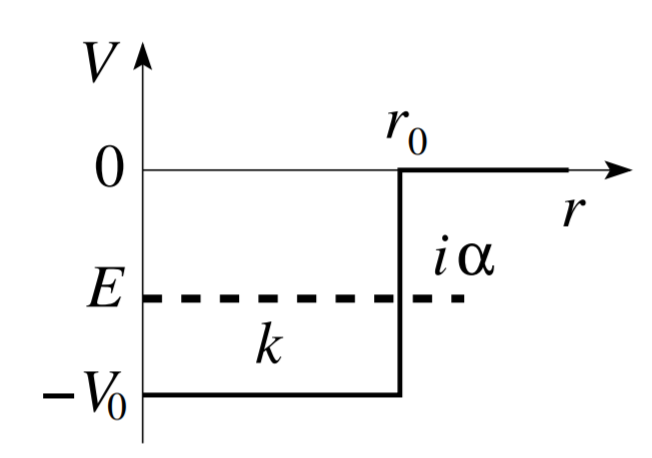
\includegraphics[scale=1]{5_3.PNG}
    \end{minipage}
    \begin{minipage}{0.5\textwidth}
        \captionsetup{font={Large}}
        \caption{Well potential of depth $V_0$ and width $r_0$.}
    \end{minipage}
\end{figure}
\subsection{For $l = 0$}
we get the differential equation
%公式 5.18
\begin{equation}
\begin{aligned}\left[\partial_{r}^{2}+k^{2}\right] u_{0}(r) &=0, \quad r \leq r_{0} \\\left[\partial_{r}^{2}-\alpha^{2}\right] u_{0}(r) &=0, \quad r \geq r_{0} \end{aligned}
\end{equation}
with the solution
%公式 5.19
\begin{equation}
\begin{array}{l}{u_{0}\left(r \leq r_{0}\right)=A e^{i k r}+B e^{-i k r}} \\ {u_{0}\left(r \geq r_{0}\right)=C e^{-\alpha r}}\end{array}
\end{equation}
The solution (5.19) must satisfy the boundary conditions at $r = 0, u_0 (0) = 0 \Rightarrow A + B = 0$, and at $r_0$,
%公式 5.20
\begin{equation}
\begin{aligned} u_{0}\left(r_{0}^{-}\right)=& u_{0}\left(r_{0}^{+}\right) \\ & \Rightarrow 2 i A \sin k r_{0}=C e^{-\alpha r_{0}} \\ u_{0}^{\prime}\left(r_{0}^{-}\right)=& u_{0}^{\prime}\left(r_{0}^{+}\right) \\ & \Rightarrow 2 i k A \cos k r_{0}=-\alpha C e^{-\alpha r_{0}} \end{aligned}
\end{equation}
We get an (3.29) equivalent implicit equation for $E$,
%公式 5.21
\begin{equation}
    \cot k r_{0}=-\frac{\alpha}{k}
    \end{equation}
We find bound states if $V0> \hbar^2\pi^2/8mr_0^2$, noting that $r_0 \longleftrightarrow w / 2$.

\subsection{For $l=0$}
we define $\rho = kr$ and get the differential equation for $r<r_0$
%公式 5.22
\begin{equation}
    \left[\partial_{\rho}^{2}+\frac{2}{\rho} \partial_{\rho}+\left(1-\frac{l(l+1)}{\rho^{2}}\right)\right] R_{l}(\rho)=0
    \end{equation}
This equation also holds for $r >r_0$ if we redefine the variable $\rho$ to $\rho\equiv i\alpha r$. The solutions of (5.22) are the verbal Bessel and Neumann functions,
%公式 5.23

%公式 5.24
\begin{align}
\text { Bessel } \rightarrow j_{l}(\rho)&=\sqrt{\frac{\pi}{2 \rho}} \mathcal{J}_{l+\frac{1}{2}}(\rho) \\
 \text { Neumann } \rightarrow n_{l}(\rho)&=(-1)^{l+1} \sqrt{\frac{\pi}{2 \rho}} \mathcal{J}_{-l-\frac{1}{2}}(\rho)
\end{align}
The Bessel functions $\mathcal{J}n$ are the solutions of the differential equation
%公式 5.25
\begin{equation}
    \left[\partial_{\varrho}^{2}=\frac{1}{\rho} \partial_{\varrho} \pm\left(1-\frac{n^{2}}{\rho^{2}}\right)\right] \mathcal{J}_{n}(\rho)=0
    \end{equation}
Note that (5.22) is less than $l+\frac{1}{2}\rightarrow -l-\frac{1}{2}$ symmetric, and thus bypasses the Neumann solutions into the Bessel solutions. Examples of the verbal Bessel and Neumann functions are (see also figure 5.4 and 5.5).

%公式 5.26
\begin{equation}
\begin{aligned} 
j_{0} &=\frac{\sin \rho}{\rho}, & n_{0} &=-\frac{\cos \rho}{\rho} \\ 
j_{1} &=\frac{\sin \rho}{\rho^{2}}-\frac{\cos \rho}{\rho}, & n_{1} &=-\frac{\cos \rho}{\rho^{2}}-\frac{\sin \rho}{\rho} \\ 
j_{2} &=\left(\frac{3}{\rho^{3}}-\frac{1}{\rho}\right) \sin \rho-\frac{3}{\rho^{2}} \cos \rho, & n_{2} &=-\left(\frac{3}{\rho^{3}}-\frac{1}{\rho}\right) \cos \rho-\frac{3}{\rho^{2}} \sin \rho
\end{aligned}
\end{equation}
%图 5.4,5.5
\begin{figure}[ht]
    \centering
    \subfigure{
        \begin{minipage}{7cm}
            \centering
            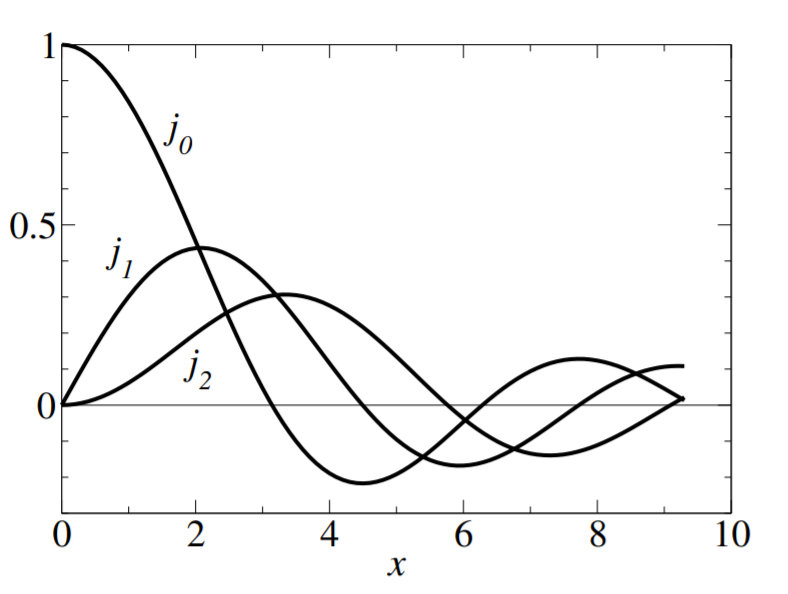
\includegraphics[scale=1]{5_4.PNG}
            \captionsetup{font={Large}}
            \caption{Bessel functions $j_0(x),j_1(x), j_2(x)$.}
        \end{minipage}
    }
    \subfigure{
        \begin{minipage}{7cm}
            \centering
            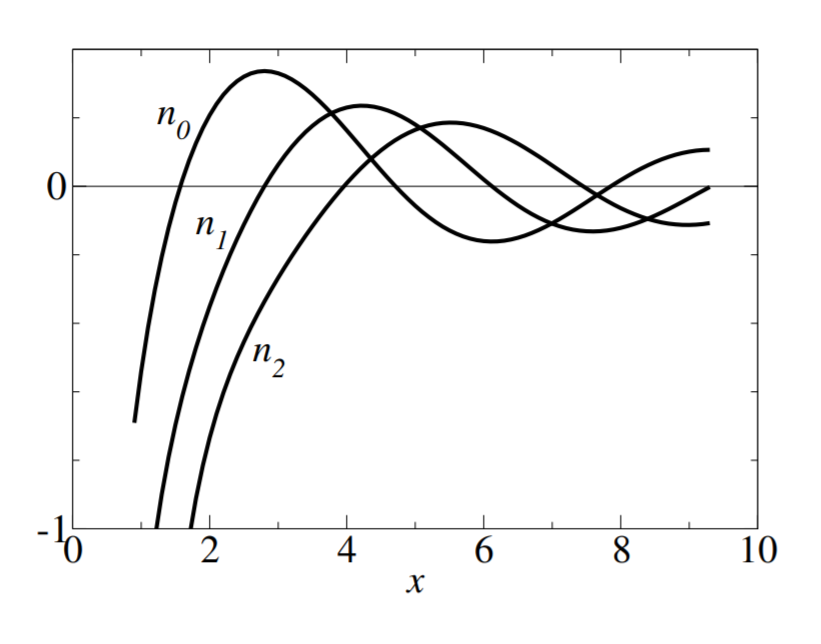
\includegraphics[scale=0.93]{5_5.PNG}
            \captionsetup{font={Large}}
            \caption{Neumann functions $n_0 (x), n_1 (x), n_2 (x)$.}
        \end{minipage}
    }
\end{figure}
\\
The spherical Bessel functions show the following behavior for small (series expansion for $\rho \rightarrow 0$) and large (asymptotic for $\rho \rightarrow \infty$) arguments:
%公式 5.
\begin{equation}
\begin{aligned} \rho & \rightarrow 0: & \rho & \rightarrow \infty \\ j_{l} & \sim \frac{\rho^{l}}{(2 l+1) ! !}, & j_{l} & \sim \frac{1}{\rho} \cos [\rho-(l+1) \pi / 2] \\ n_{l} & \sim-\frac{(2 l-1) ! !}{\rho^{l+1}},   &n_{l} &\sim \frac{1}{\rho} \sin [\rho-(l+1) \pi / 2] \end{aligned}
\end{equation}
For the spherical Bessel functions $z_l = j_l, n_l$ the recursion formulas $(l> 0)$ apply
%公式 5.28
\begin{equation}
\begin{aligned}
    z_{l-1}+z_{l+1}&=\frac{2 l+1}{\rho} z_{l}\\
    \partial_pz_l&=z_{l-1}-\frac{l+1}{\rho}z_l
\end{aligned}
\end{equation}
For $\rho\rightarrow 0$, $n_l$ is always singular, and thus it is a solution; $R_l(r>r_0)$ can then be represented as
%公式 5.29
\begin{equation}
    R_{l}\left(r \leq r_{0}\right)=A j_{l}(k r)
    \end{equation}
In the outer space $r \geq r_0$ we choose the combinations
% 5.30
\begin{equation}
\begin{aligned} h_{l}^{(1)}(\rho) &=j_{l}(\rho)+i n_{l}(\rho) \\ h_{l}^{(2)}(\rho) &=j_{l}(\rho)-i n_{l}(\rho) \end{aligned}
\end{equation}
the Hankel functions with the asymptotic behavior
%公式 5.31
\begin{equation}
    h_{l}^{(1,2)} \sim \frac{1}{\rho} e^{\pm i[\rho-(l+1) \pi / 2]}
    \end{equation}
With $\rho\equiv i\alpha r$ we obtain an exponentially decaying function for ¨$R_l (r \geq r_0)$ outside $r_0$,
%公式 5:32
\begin{equation}
\begin{aligned} R_{l}\left(r \geq r_{0}\right) &=B\left[j_{l}(i \alpha r)+i n_{l}(i \alpha r)\right] \\ &=B h_{l}^{(1)}(i \alpha r) \\ & \sim \frac{B}{\rho}(-i)^{l+1} e^{-\alpha r} \end{aligned}
\end{equation}
the component $h_l^{(2)}(kr)\propto exp[-ikr]$ was describing an incident wave, $h_l^{(2)}(i\alpha r)\propto exp[\alpha r]$ describing a non-normative solution. The energy levels are again obtained from the boundary conditions at $r = r_0$: with $\xi = kr_0$ and $\eta =\alpha r_0,\hbar k=\sqrt{2m(E+V_0)}$ and $\hbar \alpha = \sqrt{2m|E|}$ we find the relations

%公式 5:33
\begin{equation}
    \xi^{2}+\eta^{2}=2 m V_{0} r_{0}^{2} / \hbar^{2}, \quad E=-\frac{\hbar^{2}}{2 m r_{0}^{2}} \eta^{2}
    \end{equation}
The boundary conditions
%公式 5:34
\begin{equation}
    R_{l}\left(r_{0}^{-}\right)=R_{l}\left(r_{0}^{+}\right), \quad R_{l}^{\prime}\left(r_{0}^{-}\right)=R_{l}^{\prime}\left(r_{0}^{+}\right)
    \end{equation}
result in the implicit transcendental equations for $\xi$ and $\eta$ which lead to the energies $E$,
%公式 5:35
\begin{equation}
\begin{aligned} l &=0: \quad \xi \cot \xi=-\eta \\ l &=1: \quad \frac{\cot \xi}{\xi}-\frac{1}{\xi^{2}}=\frac{1}{\eta}+\frac{1}{\eta^{2}} \\ & \vdots \end{aligned}
\end{equation}
For every angular momentum sector $¨l$, a new transcendental equation $\eta(\xi)$ results. In each equation, a $\operatorname{cot} \xi$ function with an infinite number of branches appears. We number these with $n$, with the new branches appearing at $\xi = (n + 1/2) \pi$, respectively. These branches define the quantum number $n$ in the angular momentum sector $l$, thus the eigenvalues ​​depend on 2 quantum numbers, $E_{nl}$. The levels are degenerate in $m$, since the magnetic quantum number $m$ does not appear in the differential equation, but for each $l (2l + 1)$ functions $Y_{lm}$ occur, which is why each eigenvalue $E_{nl}$ is just $(2l + 1)$-fold degenerate. This is the normal degeneracy in a SO3 invariant system. The hydrogen atom will turn out to be a special case, with levels only dependent on $n, E_n \propto -1 / n^2$, and a higher degeneracy $\propto n^2$. The deeper reason for this higher degeneracy is the greater symmetry in the hydrogen problem, SO4 instead of SO3.
\\\\
New bound states appear in the $l = 0$ sector if cot $\xi$ $\rightarrow 0$, ie $\xi$ passes through the value $n\pi + \pi / 2$; the first bound state (at $E = 0^-$) appears at $\eta = 0$ and $\xi = \pi / 2$, ie $V_0 = \hbar^2\pi^2/8mr_0^2$. For $l = 1$, new states appear when cot$\xi$ becomes finite from $+ \infty$, that is, at $\xi = nπ$, where $n = 0$ does not produce a solution; the first bound state (at $E = 0 $-) then appears for $\eta \rightarrow 0, \xi \rightarrow \pi$ if $V_0 = \hbar^2\pi^2/2mr_0^2$, compare with $l = 0$ where the first state appears at $V_0 = \hbar^2\pi^2/8mr_0^2$; the repulsive centrifugal force counteracts the formation of bonded states.

\section{Hydrogen atom}
\subsection{2-body problems}
First we repeat the classical problem: Let the Hamiltonian be given for two interacting (potential $V (r = | \vec{r} |))$ massive (mass $m_{1,2}$) particles,
%公式 5:36
\begin{equation}
    H=\frac{p_{1}^{2}}{2 m_{1}}+\frac{p_{2}^{2}}{2 m_{2}}+V\left(\left|\vec{r}_{1}-\vec{r}_{2}\right|\right)
    \end{equation}
We go to center of gravity and relative coordinates $\vec{R}$ and $\vec{r}$ about\footnote{For a multiple-body problem with $n$ particles in positions $x_i, i = 1,\cdots, n$, defined one the center of gravity coordinate (COM) $nX=\Sigma_1^n x_i$ and the relative COM coordinates $\tilde{x}_i = x_i -X$, then $\Sigma_1^n \tilde{x}_i=0$. The kinetic energy $T=\Sigma_1^n\dot{x}^2_i$ then lets go to print out the relative coordinates $\delta x_{ij}=x_j-x_i=\delta\tilde{x}_{ij}, T=n\dot{X}^2+n^{-1}\Sigma_{i<j}\delta\dot{x}_{ij}^2$. To the proof write $T=x\dot{X}^2+\Sigma_1^n \tilde{\dot{x}}_i^2$ then print the equation $(\Sigma_1^n\tilde{\dot{x}}_i)^2=0$ by $\Sigma_1^n\tilde{\dot{x}}_i^2+R=0$ and eliminate the remainder $R$ via the relation $\Sigma_{i<j}\delta\dot{x}_{ij}^2=(n-1)\Sigma_1^n\tilde{\dot{x}}_i^2-R$}.
%公式 5:37
\begin{equation}
    \vec{r}=\vec{r}_{1}-\vec{r}_{2}, \quad \vec{R}=\frac{m_{1} \vec{r}_{1}+m_{2} \vec{r}_{2}}{m_{1}+m_{2}}
    \end{equation}
also for the (conjugate) impulses
%公式 5:38
\begin{equation}
    \vec{p}=\frac{m_{2} \vec{p}_{1}-m_{1} \vec{p}_{2}}{m_{1}+m_{2}}, \quad \vec{P}=\vec{p}_{1}+\vec{p}_{2}
    \end{equation}
We define the reduced and the total mass
%公式 5:39
\begin{equation}
    m=\mu=\frac{m_{1} m_{2}}{m_{1}+m_{2}}, \quad M=m_{1}+m_{2}
    \end{equation}
We quantize with the help of the commutation relations: From $[x_{\nu i},p_{\mu j}]=i\hbar\delta_{ij}\delta_{\nu\mu}$ for $\nu,\mu\in {1, 2}; i, j \in {1, 2, 3}$ follow the commutation relations for ¨ $\vec{r}$ and $\vec{p}$ and $\vec{R}$ and $\vec{P}$,
%公式 5:40
\begin{equation}
    \left[x_{i}, p_{j}\right]=i \hbar \delta_{i j}, \quad\left[X_{i}, P_{j}\right]=i \hbar \delta_{i j}
    \end{equation}
and we get the following representations for ¨ $\vec{p}$ and $\vec{P}$,
%公式 5:41
\begin{equation}
    \vec{p}=\frac{\hbar}{i} \vec{\nabla}_{\vec{r}}, \quad \vec{P}=\frac{\hbar}{i} \vec{\nabla}_{\vec{R}}
    \end{equation}
The Hamiltonian in relative and center of gravity coordinates has the shape
%公式 5:42
\begin{equation}
    H=\frac{P^{2}}{2 M}+\frac{p^{2}}{2 \mu}+V(r)
    \end{equation}
and allows the separation of center of gravity and relative movement through the approach
%公式 5:43
\begin{equation}
    \Psi_{\vec{K}}(\vec{r}, \vec{R})=e^{i \vec{K} \cdot \vec{R}} e^{-i \hbar K^{2} t / 2 M} e^{-i E t / \hbar} \psi(\vec{r})
    \end{equation}
with the remaining relative problem
%公式 5:44
\begin{equation}
    \left[\frac{p^{2}}{2 \mu}+V(r)\right] \psi(\vec{r})=E \psi(\vec{r})
    \end{equation}
The total energy is then the combination E + ~ 2K2 / 2M

\subsection{Coulomb potential, H atom}
We solve the relative problem
% 5:45
\begin{equation}
    \left[-\frac{\hbar^{2}}{2 m} \vec{\nabla}^{2}+V(r)\right] \psi(\vec{r})=E \psi(\vec{r})
    \end{equation}
with the Coulomb potential $V (r) = -Z e^2 / r$. After the separation of the angle coordinates $[\psi (\vec{r}) = \psi (r, \theta, \varphi) = Y_{l, m}(\theta, \varphi) R_{\alpha l} (r)]$ and using the approach $R_{\alpha l} = u_{\alpha l} / r$, we obtain the radial problem
%公式 5:46
\begin{equation}
    \left[\partial_{\rho}^{2}-\frac{l(l+1)}{\rho^{2}}+\frac{2}{\rho}-\alpha^{2}\right] u_{\alpha l}(\rho)=0
    \end{equation}
Here we have the length scale
%公式 5:47
\begin{equation}
    a_{B}=\hbar^{2} / m_{e} e^{2}=0.529 \mathrm{A}
    \end{equation}
We introduce ($\rho = Zr / a_B$, we approximate $m \approx m_e$ because $M\gg m_e$ of the hydrogen problem) and rewrite the energy $E$ according to the scaling
%公式 5:48
\begin{equation}
    \alpha^{2}=\frac{-E}{Z^{2} E_{R}}, \quad E_{R}=\frac{\hbar^{2}}{2 m_{e} a_{B}^{2}}=13.605 \mathrm{eV}
    \end{equation}
$a_B$ is called Bohr radius, $E_R$ is the Rydbergen energy; they are the relevant length and energy scales in the problem. After the usual splitting off of the asymptotic (for $\rho \rightarrow 0, \infty$) we use the Fuchsian approach (see (5.13) and (5.16))
%公式 5:49
\begin{equation}
\begin{aligned} u_{\alpha l}(\rho) &=\rho^{l+1} e^{-\alpha \rho} f_{\alpha l}(\rho) \quad \text { with } \\ f_{\alpha l}(\rho) &=\sum_{\nu} a_{\nu} \rho^{\nu} \end{aligned}
\end{equation}
and get the differential equation
%公式 5:50
\begin{equation}
    \partial_{\rho}^{2} f_{\alpha l}+2\left(\frac{l+1}{\rho}-\alpha\right) \partial_{\rho} f_{\alpha l}+\frac{2}{\rho}[1-\alpha(l+1)] f_{\alpha l}(\rho)=0
    \end{equation}
The coefficient comparison in the powers $\rho^{\nu}$ gives the recursion

%公式 5:51
\begin{equation}
    a_{\nu+1}=2 \frac{\alpha(l+\nu+1)-1}{(\nu+1)(\nu+2 l+2)} a_{\nu}, \quad \nu=0,1,2, \ldots
    \end{equation}
%表 5.1
\begin{table}
    \centering
    \captionsetup{font={Large}}
    \Large
    \begin{tabular}{c|c|c}

        \hline
        End level & Name & Energy\\
        \hline
        n=1 & Lyman & UV \\
        n=2 & Balmer & Visible\\
        n=3 & Paschen & IR \\
        n=4 & Bracket & IR\\
        n=5 & Pfund & IR \\
        \hline
    \end{tabular}
    \caption{Transition between levels}
\end{table}
\\
The coefficient $a_0$ is determined by normalization. Since $a_{\nu + 1} / a_{\nu} \sim 2\alpha / \nu, \nu \rightarrow \infty$, the series must break off and we get the spectrum
%公式 5:52
\begin{equation}
    \alpha = \frac{1}{l+1+\nu}
\end{equation}
The eigenvalues
%公式 5:53
\begin{equation}
    E_{n}=-\frac{Z^{2} E_{R}}{n^{2}}, \quad n=1,2,3, \ldots=\text { Principal quantum number }
    \end{equation}
occur with the degrees of degeneration $D_n$
%公式 5:54
\begin{equation}
    D_{n}=\sum_{m, l, \nu} \delta_{l+1+\nu, n}=\sum_{l=0}^{n-1}(\underbrace{2 l+1}_{\Sigma_{m}})=n^{2}
    \end{equation}
\\
The quantum numbers $n, l, m$ are called the main quantum number $n$, the minor or orbital angular momentum quantum number $l$, and the magnetic quantum number $m$. The additional degeneracy in $l$ is a consequence of the dynamic symmetry in the Coulomb potential. If the spin is taken into account (see later) the degeneration doubles, $D_n = 2n^2$. The transitions between the levels involve $\Delta l = 1$ (see later) and belong to one of the sequences in table 5.1; see also figure 5.6 for a graphical representation of the states involved.

\subsection{Radial wave functions}
The radial wave functions of the Coulomb potential result from the differential equation (5.50), which we use via the manipulations
%公式 5:55
\begin{equation}
    \partial_{\rho}^{2}+2[(l+1) / \rho-\alpha] \partial_{\rho}+(2 / \rho)[1-\alpha(l+1)]
    \end{equation}
%表 5.6
\begin{figure}[ht]
    \centering
    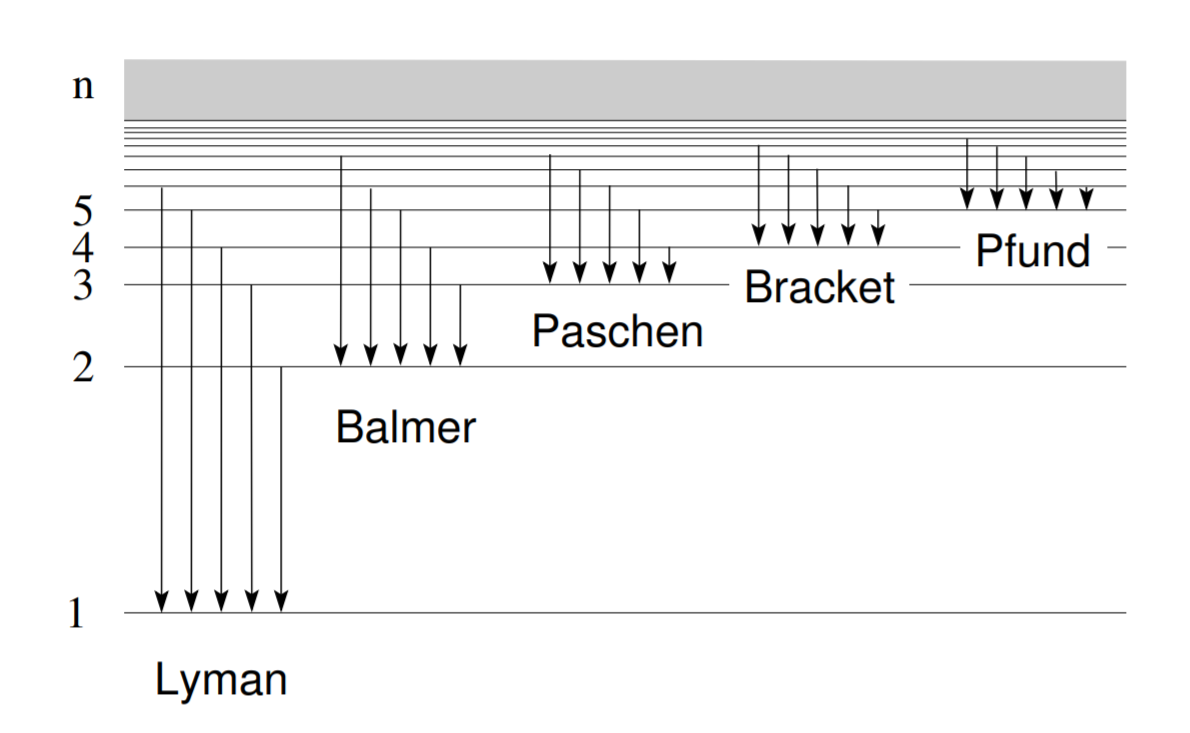
\includegraphics[scale=1]{5_6.PNG}
    \captionsetup{font={Large}}
    \caption{U-tops in the H-atom: Lyman, Balmer, Paschen, Bracket and Pound series. The Lyman series is in the UV range with energies greater than 10 eV; the Balmer series is in the visible range with energies in the range of greater 1.9 eV (red, cyan, violet); the Paschen series is in the IR range with energies greater than 0.65 eV.}
\end{figure}
%公式 5:56

%公式 5:57
\begin{eqnarray}
\begin{aligned} 
\downarrow & z=2 \alpha \rho \\ 
4 \alpha^{2} \partial_{z}^{2}+4 \alpha[2 \alpha(l+1) / z-\alpha] & \partial_{z}+(4 \alpha / z)[1-\alpha(l+1)] 
\end{aligned}
\end{eqnarray}
\begin{equation}
    \begin{aligned}
        & \downarrow \cdot z / 4 \alpha^{2} \\ 
z \partial_{z}^{2}+[\underbrace{2(l+1)}_{b}-&z] \partial_{z}+[\underbrace{1 / \alpha-(l+1)}_{-a}] 
    \end{aligned}
\end{equation}
into the following form ($n = 1 / \alpha$)
%公式 5:
\begin{equation}
    \left\{z \partial_{z}^{2}+[2(l+1)-z] \partial_{z}+[n-(l+1)]\right\} f_{n l}(z)=0
    \end{equation}
The comparison with the differential equation
%公式 5:59
\begin{equation}
    z \partial_{z}^{2} F+(b-z) \partial_{z} F-a F=0
    \end{equation}
with the solutions (confluent hypergeometric functions)
%公式 5.60
\begin{equation}
    F(a, b ; z)=1+\frac{a}{b 1 !} z+\frac{a(a+1)}{b(b+1) 2 !} z^{2}+\cdots
    \end{equation}
gives us the radial functions in the form
%公式 5.61
\begin{equation}
\begin{aligned} R_{n l}\left(r=\rho a_{B} / Z\right) &=\rho^{l} e^{-\alpha \rho} f_{n l}(z=2 \rho / n) \\ & \propto(\kappa r)^{l} e^{-\kappa r} F(-n+l+1,2 l+2 ; 2 \kappa r) \end{aligned}
\end{equation}
with $z = 2\alpha\rho = 2Z r / n a_B = 2\kappa r, \kappa = Z / a_Bn$ the effective wavenumber. The boundary condition (for $r\rightarrow\infty$) requires that $n-l-1 = ν \geq 0$ is an integer, resulting in the spectrum $E = -\hbar^2/2m_ea^2_Bn^2=-m_ee^4/2\hbar^2n^2,n\in\mathbb{N}$. The confluent hypergeometric function with integer parameters is (except for one factor) identical to the associated Laguerre polynomial
\footnote{The Laguerre differential equation
%公式 5.62
\begin{equation}
    \left[z \partial_{z}^{2}+(1-z) \partial_{z}+p\right] L_{p}(z)=0, \quad p>0
    \end{equation}
is solved by the Laguerre polynomials
%公式 5.63
\begin{equation}
    L_{p}(z)=e^{z} \partial_{z}^{p}\left(z^{p} e^{-z}\right), \quad p=0,1, \ldots
    \end{equation}
The following recursion formulas apply to $L_p (z)$
%公式 5.64
\begin{equation}
\begin{aligned} L_{p+1} &=(2 p+1-z) L_{p}-p^{2} L_{p-1} \\ \partial_{z} L_{p} &=p\left(\partial_{z} L_{p-1}-L_{p-1}\right) \end{aligned}
\end{equation}
The assigned Laguerre polynomial
%公式 5.65
\begin{equation}
    L_{p}^{k}(z)=\partial_{z}^{k} L_{p}(z)=\frac{p !}{(p-k) !} e^{z} \partial_{z}^{p}\left(z^{p-k} e^{-z}\right)
    \end{equation}
solve the differential equation
%公式 5.66
\begin{equation}
    \left[z \partial_{z}^{2}+(k+1-z) \partial_{z}+(p-k)\right] L_{p}^{k}(z)=0, \quad k \leq p
    \end{equation}}
%公式 5.67
%\begin{equation}
\begin{align}
L_{p}^{k}(z)&=\frac{p !}{(p-k) !} e^{z} \partial_{z}^{p}\left(z^{p-k} e^{-z}\right)\\
  %  \end{equation}
%公式 5.68
%\begin{equation}
F(-p+k, k+1 ; z) &\propto L_{p}^{k}(z)
\end{align}
%\end{equation}
and the identification $p = n + 1, k = 2l + 1$ gives us the following final results for the generalized hydrogen atom,
% 5.69

%公式 5.70
%\begin{equation}
\begin{align} 
    \Psi_{n l m}(r, \theta, \varphi) &=R_{n l}(r) Y_{l m}(\theta, \varphi) \\ 
    R_{n l}(r) &=-N_{n l}(2 \kappa r)^{l} e^{-\kappa r} L_{n+l}^{2 l+1}(2 \kappa r) \\
    N_{n l} &=\left(\frac{Z}{a_{B}}\right)^{\frac{3}{2}} \frac{2}{n^{2}(n+l) !} \sqrt{\frac{(n-l-1) !}{(n+l) !}}\notag
 \end{align}
%\end{equation}
The radial function is normalized to 1,
%公式 5.71
\begin{equation}
    \int_{0}^{\infty} d r r^{2}\left|R_{n l}(r)\right|^{2}=1
    \end{equation}
which is via the integral
%公式 5.72
\begin{equation}
    \int_{0}^{\infty} d z z^{k+1} \mathrm{e}^{-z}\left[L_{p}^{k}(z)\right]^{2}=\frac{(p !)^{3}}{(p-k) !}(2 p-k+1)
    \end{equation}
the normalization constant $N_{nl}$ yields. Explicit examples of radial functions with $n \leq 3$ are (see also figure 5.7)

%公式 5.73
\begin{equation}
\begin{aligned} R_{10} &=2 \kappa^{3 / 2} \exp [-\kappa r] \\ R_{20} &=2 \kappa^{3 / 2}(1-\kappa r) \exp [-\kappa r] \\ R_{21} &=\frac{2 \kappa^{3 / 2}}{\sqrt{3}} \kappa r \exp [-\kappa r] \\ R_{30} &=2 \kappa^{3 / 2}\left[1-2 \kappa r+2(\kappa r)^{2} / 3\right] \exp [-\kappa r] \\ R_{31} &=\frac{4 \sqrt{2} \kappa^{3 / 2}}{3} \kappa r(1-\kappa r / 2) \exp [-\kappa r] \\ R_{32} &=\frac{2 \sqrt{2} \kappa^{3 / 2}}{3 \sqrt{5}}(\kappa r)^{2} \exp [-\kappa r] \end{aligned}
\end{equation}
With increasing principal quantum number $n$, the orbit $\langle r\rangle_{nl}$ shift outwards
%公式 5.74
\begin{equation}
    \langle r\rangle_{n l}=\frac{a_{B}}{2 Z}\left(3 n^{2}-l(l+1)\right)
    \end{equation}
and the fluctuations $\Delta r=[\langle r^2\rangle_{nl}-\langle r\rangle^2_{nl}]^{1/2}$ grow according to
%公式 5.75
\begin{equation}
    \Delta r=\frac{a_{B}}{2 Z} \sqrt{n^{2}\left(n^{2}+2\right)-l^{2}(l+1)^{2}}
    \end{equation}
where we used that
%公式 5.76
\begin{equation}
    \left\langle r^{2}\right\rangle_{n l}=\frac{n^{2} a_{B}^{2}}{2 Z^{2}}\left[5 n^{2}-3 l(l+1)+1\right]
    \end{equation}
Finally, we consider the characteristics of two particularly simple cases, $l = n - 1$ and $l = 0$. For $¨l = n - 1$, the radial function $R_{n, n-1}$ has no zeros and their characteristics are
%公式 5.77
\begin{equation}
\begin{aligned}\langle r\rangle_{n, n-1} &=\frac{a_{B}}{2 Z} n(2 n+1) \\ \Delta r_{n, n-1} &=\frac{a_{B}}{2 Z} n \sqrt{2 n+1} \\ \Delta r /\left.\langle r\rangle\right|_{n, n-1} & \sim 1 / \sqrt{2 n+1} \rightarrow 0 \text { für } n \rightarrow \infty \end{aligned}
\end{equation}
%图 5.7
\begin{figure}[ht]
    \begin{minipage}{0.5\textwidth}
        \centering
        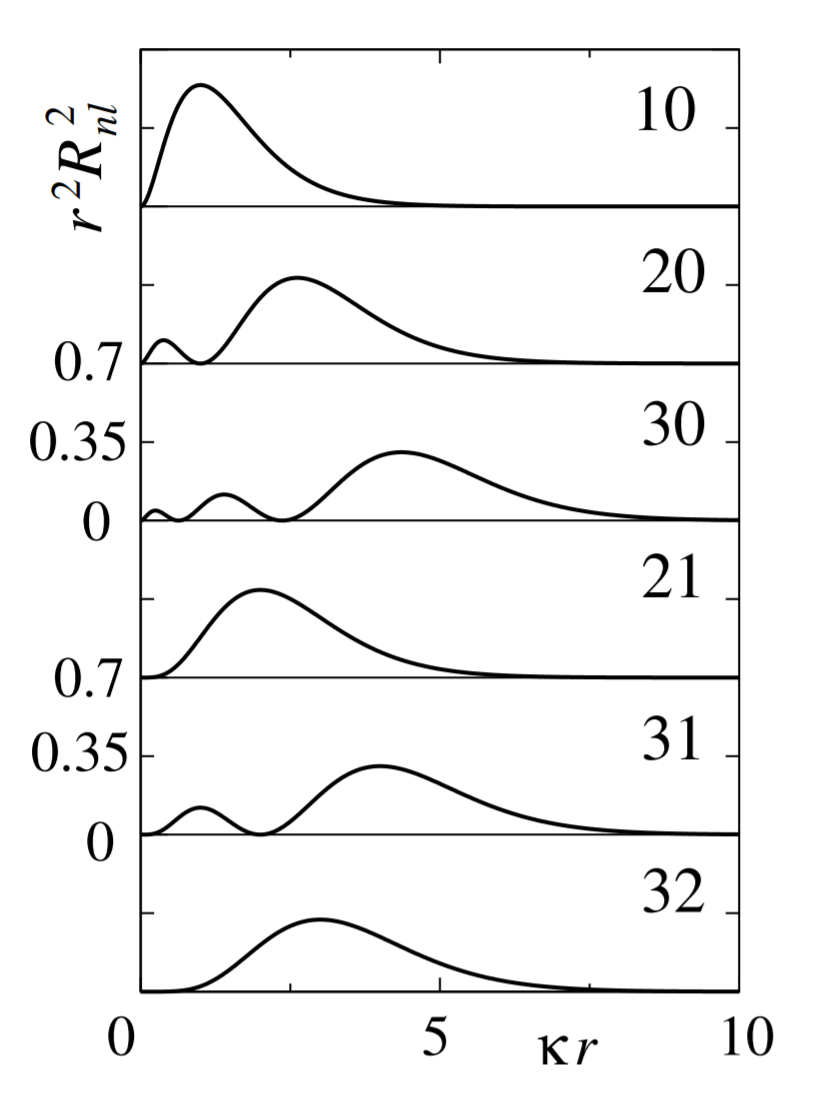
\includegraphics[scale=1]{5_7.PNG}
    \end{minipage}
    \begin{minipage}{0.5\textwidth}
        \captionsetup{font={Large}}
        \caption{Radial probability densities $r^2R^2_{nl}$. Note the increasing displacement of the wave function        from the environment of $r = 0$
        with $l$ ($\leftarrow$ centrifugal barrier)
        and the increase of zeros with $n$; the number zero is by $n - l - 1$
        given. The radial function
        $R_{nn-1}=[(2\kappa)^{3/2}/\sqrt{(2n)!}](2\kappa r)^{n-1}e^{-\kappa r}$ with the
        highest $l$ does not have any zero and defines for $n \rightarrow \infty$ sharp tracks (i.e.  $\Delta r / r \rightarrow 0$) at $r\sim a_B n^2/Z$.}
    \end{minipage}
\end{figure}
\\
For $¨l = 0, R_{n0}$ has the maximum number of $n - 1$ zeros and their characteristics are

%公式 5.78
\begin{equation}
\begin{aligned} R_{n 0}(0) & \neq 0 \\\langle r\rangle_{n, 0} &=\frac{3 a_{B}}{2 Z} n^{2} \\ \Delta r /\left.\langle r\rangle\right|_{n, 0} &=\sqrt{1+\left(2 / n^{2}\right) / 3} \sim 1 / 3 \end{aligned}
\end{equation}
\subsection{Dynamic Symmetry}
The dynamic symmetry is based on a special form of the law of force (the potential), here $V (r) \propto 1 / r$. A potential $1 / r^{1 + \varepsilon}, \varepsilon \neq 0$ has the geometric rotational symmetry, but not an additional dynamic symmetry. In the case of the H atom, dynamic symmetry has a classical analogue, the (obtained) lenz vector. This is not always the case: quantum-mechanically dynamic symmetry does not necessarily have to be a classical analogue. We investigate the Kepler problem $H = p^2 / 2\mu - \kappa / r$, where $\mu$ denotes the reduced mass and $\kappa$ for the generalized hydrogen atom is chosen to $\kappa = Ze^2$. Classical orbits are closed ellipses (see figure 5.8) with semiaxes $a$ and $b$ and eccentricity $e = (1 - b^2/a^2)^{1/2}$ conservation laws are the energy $E = -\kappa / 2a$ and the angular momentum $\vec{L}$, the direction $\hat{L}$ lays the orbital plane, the amount $L$ determines the eccentricity via $L^2 = \mu\kappa a (1 - e^2)$ .The trajectory is thus defined by the conserved quantities $E$ and $\vec{L}$ In addition to $H$ and $\vec{L}$ the lenticular Get Runge Vector $\vec{M}$,

%公式 5.79
\begin{equation}
\begin{aligned} \vec{M} &=\frac{1}{\mu} \vec{p} \wedge \vec{L}-\frac{\kappa}{r} \vec{r}, \quad M=\kappa e, \quad \vec{L} \cdot \vec{M}=0 \\ M^{2} &=\frac{2 H}{\mu} L^{2}+\kappa^{2} \end{aligned}
\end{equation}
$\vec{M}$ = const. implies the absence of perihelion rotation, a peculiarity of the $1 / r$-potential.
%图 5.8
\begin{figure}[ht]
    \begin{minipage}{0.5\textwidth}
        \centering
        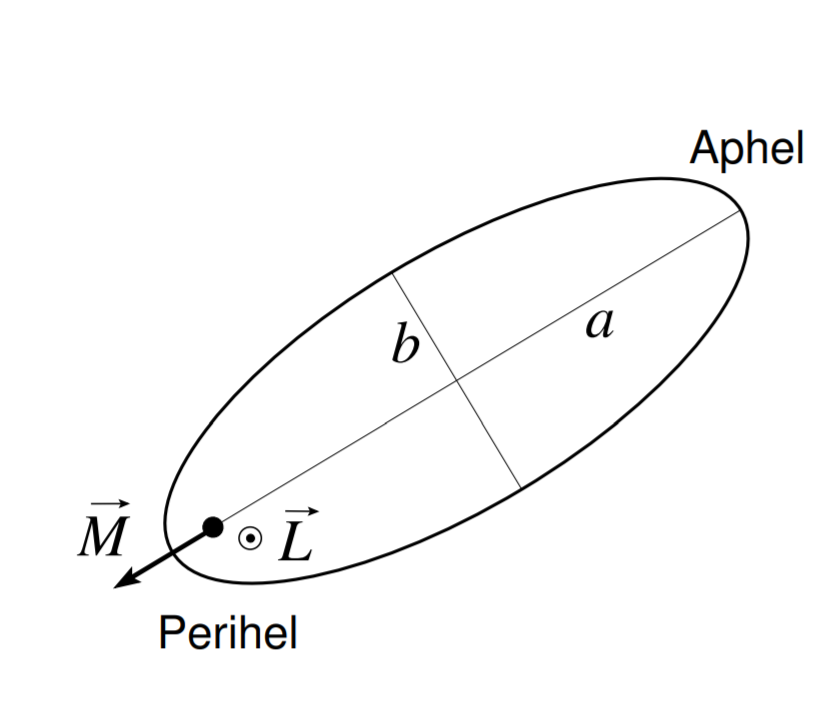
\includegraphics[scale=0.8]{5_8.PNG}
    \end{minipage}
    \begin{minipage}{0.5\textwidth}
        \captionsetup{font={Large}}
        \caption{The Runge-Lenz vector $\vec{M}$ shows from the focal point to the perihelion and is a preserved size in the Kepler problem. Perturbations of the $1 / r$-potential cause a rotation of $\vec{M}$; the observation of the peri-turn of Mercury was one of the first experimental confirmations of ART.}
    \end{minipage}
\end{figure}
Fur $V\propto1/r^{1+\varepsilon}$ results in a perihelion rotation; a famous example is the corrections to the Kepler problem as a result of the General Relativity Theory (ART); Mercury's peri-rotation was one of the first experimental confirmations of ART. The isotropic harmonic oscillator with $r^2$ potential also has a dynamic symmetry: In the isotropic harmonic oscillator, the obtained size is not a vector but a quadrupole, because center of attraction is not a focal point but the center of the elliptical orbit.
In quantum mechanics we define the Pauli-Lenz vector
%公式 5.80
\begin{equation}
    \vec{M}=\frac{1}{2 \mu}(\vec{p} \wedge \vec{L}-\vec{L} \wedge \vec{p})-\kappa \frac{\vec{r}}{r}
    \end{equation}
It is still $\vec{M}\cdot\vec{L} = 0 = \vec{L}\cdot\vec{M}$ as well
%公式 5.81
\begin{equation}
    M^{2}=2 H\left(L^{2}+\hbar^{2}\right) / \mu+\kappa^{2}
    \end{equation}
with the additional term $\propto \hbar^2$. $\vec{M}$ is a vector, so the exchange relationships apply
%公式 5.82
\begin{equation}
    \left[L_{i}, M_{j}\right]=i \hbar \varepsilon_{i j k} M_{k}
    \end{equation}
The permutation of the components $M_i$ among each other
%公式 5.83
\begin{equation}
    \left[M_{i}, M_{j}\right]=-(2 H / \mu) i \hbar \varepsilon_{i j k} L_{k}
    \end{equation}
We define $\vec{K}=\sqrt{-\mu/2H}\vec{M}$ and constrain $\vec{M}$ to $\operatorname{Eig}_{E <0}H$, $\vec{K}=\sqrt{\mu/2|E|}\vec{M}$; for $¨E <0, \vec{K}$ is a Hermitian operator. The six operators {$\vec{K},\vec{L}$} satisfy the commutation relations
%公式 5.84
\begin{equation}
\begin{aligned}\left[K_{i}, K_{j}\right] &=i \hbar \varepsilon_{i j k} L_{k} \\\left[L_{i}, K_{j}\right] &=i \hbar \varepsilon_{i j k} K_{k} \\\left[L_{i}, L_{j}\right] &=i \hbar \varepsilon_{i j k} L_{k} \end{aligned}
\end{equation}
Extend the variables $x_i, p_i, i \in {1, 2, 3}$ to $x_4, p_4$ by asking for it
%公式 5.85
\begin{equation}
\begin{aligned} L_{i j} &=r_{i} p_{j}-r_{j} p_{i}, \quad i \in\{1,2,3,4\} \\ L_{14} &=K_{x}, \quad L_{24}=K_{y}, \quad L_{34}=K_{z} \quad\left(\leftrightarrow x_{4} \& p_{4}\right) \end{aligned}
\end{equation}
thus the $L_{ij}, i \in {1, 2, 3, 4}$ form the Lie algebra of O(4). We find that the symmetry group of $H$ is not SO(3) but the larger group SO(4). For $¨E> 0$ we get the Poincare (or Lorentz) group over $\mathbb{M}^4 = (t, \vec{r}$), the Minkowski space, instead of SO(4). 
\\\\
Finally we compute the spectrum to H: using (5.81) we can write H as
%公式 5.86
\begin{equation}
    H=-\frac{\mu \kappa^{2}}{2\left(K^{2}+L^{2}+\hbar^{2}\right)}
    \end{equation}
The two vector operators
%公式 5.87
\begin{equation}
    \vec{S}=\frac{1}{2}(\vec{L}+\vec{K}) \quad \text { and } \quad \vec{D}=\frac{1}{2}(\vec{L}-\vec{K})
    \end{equation}
define the two Casimir operators\footnote{The Casimir operator is a bilinear combination of the generators of a LieAlgebra that commutes with these generators. The number of independent Casimir Operators equals the rank of the group, i.e., the maximum number of commuting generatrix. As an example consider the group SO(3) with $[L_i, L_j] = i\hbar \varepsilon_{ijk}L_k$. your Rank is 1, the Casimir operator is $L^2$, Another example is SO(4), where ${S_i, D_j}$ stands for $i$ and $j$ form a maximum commuting set. The rank is 2, the Casimir operators are $D^2$ and $S^2$,} $S^2$ and $D^2$ to SO(4):
%公式 5.88
\begin{equation}
\begin{aligned}
    \left[S_{i}, S_{j}\right]&=i \hbar \varepsilon_{i j k} S_{k}, &\left[D_{i}, D_{j}\right] &=i \hbar \varepsilon_{i j k} D_{k} \\
    [\vec{S}, \vec{D}]&=0 \longrightarrow &\left[S^{2}, \vec{S}\right]&=\left[S^{2}, \vec{D}\right] =0 \\ 
    & &\left[D^{2}, \vec{S}\right] &=\left[D^{2}, \vec{D}\right]=0 \end{aligned}
\end{equation}
$\vec{D}$ and $\vec{S}$ each define an SO(3) or SU(2) algebra. Allowed eigenvalues ​​are
%公式 5.89
\begin{equation}
\begin{aligned} \operatorname{Eig} D^{2} &=\hbar^{2} d(d+1) \\ \operatorname{Eig} S^{2} &=\hbar^{2} s(s+1) \\ d, s & \in\left\{0, \frac{1}{2}, 1, \frac{3}{2}, 2, \frac{5}{2}, \cdots\right\} \end{aligned}
\end{equation}
Since neither $\vec{S}$ nor $\vec{D}$ are orbital angular momenta, half-integer values ​​for $d$ and $s$ are allowed. It is
%公式 5.90
\begin{equation}
\begin{aligned} H &=-\frac{\mu \kappa^{2}}{2\left[(\vec{S}-\vec{D})^{2}+(\vec{S}+\vec{D})^{2}+\hbar^{2}\right]} \\ &=-\frac{\mu \kappa^{2}}{2\left(2 S^{2}+2 D^{2}+\hbar^{2}\right)} \end{aligned}
\end{equation}
Since $\vec{K}\cdot\vec{L} = 0, (\vec{S} - \vec{D}) · (\vec{S} + \vec{D}) = S^2 - D^2 = 0$, so $d = s$ and we get the energy eigenvalues

%公式 5.91
\begin{equation}
\begin{aligned} E_{n} &=-\frac{\mu \kappa^{2}}{2 \hbar^{2}[4 s(s+1)+1]} \\ &=-\frac{\mu \kappa^{2}}{2 \hbar^{2}(2 s+1)^{2}} \\ &=-\frac{\mu \kappa^{2}}{2 \hbar^{2} n^{2}} \end{aligned}
\end{equation}
with $n = (2s + 1)$ completely; the dimension of the energy eigenspace is dim $\operatorname{Eig}_{E_n}H = (2s + 1) (2d + 1) = n^2$.